\section{Introduction}

With advancements in networked multi-agent technology, multi-robot systems (MRSs) have rapidly developed towards autonomy, offering various applications from warehouse automation to search and rescue operations~\cite {6303906,1335496}. A core element of these systems is a formation controller that enables the robots to collaborate in a desired configuration~\cite{1545539,Oh2015}. In rigid formation control, achieving the desired configuration involves setting a specific target distance for each swarm agent. However, with the increasing complexity of formation tasks, the formation configuration needs to be adjustable to meet specific task requirements. Time-varying formation (TVF) control thus has become essential for swarm robots~\cite{Dong2015,Dong2016}.

\begin{figure}
\centering
\begin{subfigure}[b]{0.4\textwidth}
    
    \centering
    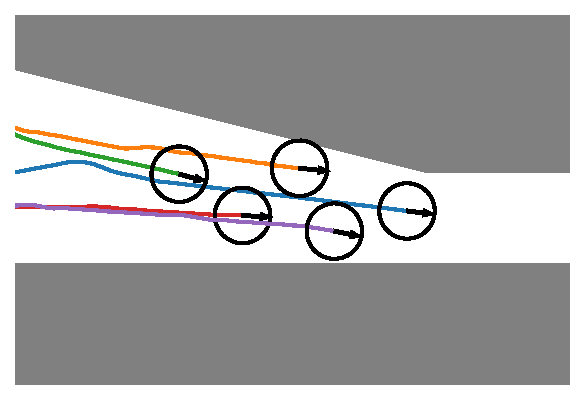
\includegraphics[width=\linewidth]{paper2/images/sample_bc.pdf}
    \caption{Pure formation control}
    \label{fig:1sample_bc}
\end{subfigure}
\begin{subfigure}[b]{0.4\textwidth}
    \centering
    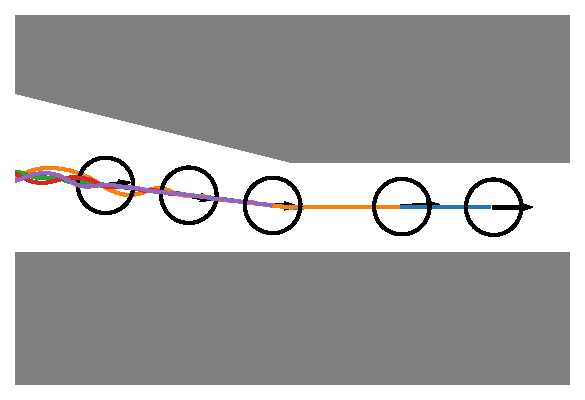
\includegraphics[width=\linewidth]{paper2/images/sample_edc.pdf}
    \caption{Proposed approach}
    \label{fig:1sample_edc}
\end{subfigure}
\caption{We develop an event-based reconfiguration control (ERC) method to guide a TVF through narrow spaces. \textit{Left:} Motion path of the TVF using purely behavior-based formation control~\cite{736776, Vsrhelyi2018}, which is collision with surrounding obstacles. \textit{Right:} Motion path of the TVF using our proposed approach, which safely navigates through the narrow spaces.}
\label{fig:1sample}
\end{figure}

Studies in~\cite{736776,Reynolds1987,Antonelli2009} show that biological swarm motion can be characterized by three primary behavioral rules: (i) \textit{cohesion}, which drives an agent toward to its neighbors; (ii) \textit{repulsion}, which pushes an agent away from its neighbors to prevent collisions; and (iii) \textit{alignment}, which aligns an agent to the dominant heading of its neighbors. For goal-oriented swarm motion, \textit{alignment} can be replaced by a \textit{migration} behavior so that each agent is directed in a desired orientation and moves at a preferred speed~\cite{6095129}. In complex environments, a fourth behavior called \textit{collision avoidance} can be added to guide the agent around obstacles~\cite{9565893, 9990164,1605401,10417519}. These behavioral rules are typically integrated into multi-robot systems through virtual forces within the artificial potential field (APF) to achieve coordinated movements~\cite{9981858,9561902,9990164}. Specifically, the APF has been used in~\cite{10417519,8716301,9565893} to navigate robot swarms through different environments, from open spaces to environments containing concave obstacles. In~\cite{9565893}, a fuzzy controller is added to allow the robot swarm to avoid complex obstacles while maintaining swarm connectivity. In~\cite{Vsrhelyi2018}, evolutionary optimization is combined with a behavioral model to enable stable and decentralized navigation for large-scale aerial robot swarms in confined spaces. However, using a fixed set of behaviors limits the flexibility of the swarm formation in response to abrupt changes in the environment, especially in spaces such as caves, corridors, and tunnels, and hence increases the risk of collisions~\cite{Saska2020,AlonsoMora2017}.

Apart from the behavior-based approach, studies in formation control can be further grouped into two primary categories: \textit{rigid formation}~\cite{Saska2020,Gmez2013,Roy2018,Ebel2017} and \textit{adaptive formation}~\cite{Fu2020,8843165,AlonsoMora2017,AlonsoMora2018}. In \textit{rigid formation}, the swarm can shrink or expand in size while preserving its overall shape. In~\cite{Saska2020}, a model predictive control is employed for rigid formation in which optimal control signals are generated for each robot in the swarm based on a shared map. In~\cite{Roy2018}, a region-based hierarchical control method is introduced for obstacle avoidance in confined spaces. The controller drives the robots to move cohesively within a virtual circular region that can contract to navigate around obstacles. A comprehensive control scheme is presented in~\cite{Ebel2017} for omnidirectional mobile robots to transport a plate through unknown environments collaboratively. The scheme uses graph-based path planning for obstacle avoidance and distributed model predictive control for optimal motion. Although rigid formations work well in open-space environments, they become ineffective in narrow spaces where the width of the space and the size of the formation directly affect navigation success. This challenge becomes critical when contracting the formation increases the risk of collision among the robots, as illustrated in Figure~\ref{fig:1sample_bc}.

In \textit{adaptive formation}, the swarm can transform into different configurations in adaptation to environmental conditions. In~\cite{Fu2020}, a reconfiguration strategy is combined with behavioral control for swarm navigation in dynamic environments. The strategy uses an auction-based market approach to generate solutions for formation movement. In~\cite{8843165}, particle swarm optimization is used to generate trajectories for a swarm of unmanned aerial vehicles (UAVs) that can reconfigure its formation for obstacle avoidance and task accomplishment. However, this approach is centralized and requires considerable computational resources to maintain an optimal configuration in real time. A robust adaptive formation control algorithm is introduced in~\cite{Mung2019} for a group of UAVs. The controller can steer the vehicles to form and maintain different formation patterns for flexible navigation. Generally, the adaptive formation methods are effective in guiding robots through complex environments as they enable flexible reconfiguration in response to environmental changes. However, there remains a need for a distributed, partial communication solution that ensures safe, efficient formation navigation while adapting effectively to environmental change.

In this work, we propose an event-based reconfiguration controller (ERC) for safe and effective navigation of a decentralized TVF in narrow environments, as given in Figure~\ref{fig:1sample}. The robots are equipped with local sensors and communication modules to collect information about the environment and other robots in the formation. The main contributions of this study are threefold:
\begin{enumerate}
    \item Define a set of individual behaviors that meet the reconfiguration control requirements, including goal-directed motion, formation maintenance, tailgating, and collision avoidance behaviors. Each behavior is designed for convenience in implementation via an artificial potential field.
        \item Propose an event-based reconfiguration controller with two modes, \textit{``formation''} and \textit{``tailgating''} capable of adapting the formation shape in response to environmental changes. The stability of the proposed approach has been demonstrated via the Lyapunov theorem.
    \item Extensive simulations and comparisons have been conducted to evaluate the robustness, scalability, and effectiveness of the proposed controller. Software-in-the-loop tests have also been conducted to verify its practical applicability. The source code of the proposed controller is publicly available for further research and practical implementation.
\end{enumerate}

The remaining sections of this paper are organized as follows. Section~\ref{sec2} presents the formation model and formulation. Section~\ref{sec3} introduces the proposed event-based reconfiguration control method. Simulation, comparison, and software-in-the-loop experimental results are shown in Section~\ref{sec4}. The paper ends with conclusions drawn in Section~\ref{sec5}.